% Document settings
\documentclass[11pt]{article}
% % % % % % % % % % % Define Footer
\usepackage{fancyhdr}
\usepackage[margin=1in]{geometry}
\usepackage[pdftex]{graphicx}
\usepackage{multirow}
\usepackage{setspace}
\pagestyle{plain}
\usepackage[american voltages,oldvoltagedirection]{circuitikz}
%\usepackage[american]{circuitikz}
\usepackage{graphicx}
\usepackage{multirow}
\usepackage{booktabs}
\usepackage{epstopdf}
%\usepackage{MnSymbol,wasysym}
\usepackage{amsmath}
%\usepackage{mathtools}
\usepackage{amssymb}
\usepackage{lipsum}
\usepackage{siunitx}
\setlength\parindent{0pt}
\graphicspath{{images/}{drawings/}}
\usepackage{float}
% % % % % % % % % % % Header footer
% % % % % % % % % % %EDIT THIS % % % % % % % % % % % % % % % % % % % %
\pagestyle{fancy}
\fancyhf{}
\lhead{Tech Memo: Experiment 4-Operational Amplifiers}
\rhead{Andrei Tumbar}
\lfoot{EE281}
\cfoot{4/7/20}
\rfoot{Page \thepage}
% % % % % % % % % % % % % % % % % % % % % % % % % % % % % % % % % % % % %

\begin{document}
	\numberwithin{equation}{subsection}
	\numberwithin{figure}{subsection}
	\numberwithin{table}{subsection}
	\hspace{6in}
		
\includegraphics[scale=0.9,trim=0cm 0in 0in 0.0in,clip]{RIT_KGCOE1}
\newline

\Huge \textbf{EEEE 281 Experiment 4:\\ Operational Amplifiers}\\

\Large
\textbf{From:}Andrei Tumbar [Computer Engineering] \\
\textbf{To: } Section 2 TA: LJ Boone \\
\textbf{Date: } Performed: 4/7/20  Due: 4/14/20 \\
\textbf{Subject: } Lab 4-Operational Amplifiers\\
\textbf{Lab Partner(s): } N/A\\
\vspace{0.5in}
	\begin{table}[h!]
		\centering
		%\caption{Grading Table}
		%\label{Table:Grading Table 1}
		%\begin{tabular}{llllll}
		\begin{tabular}{|l||l|l|l|l|}
			\hline
			Component & Percentage of Grade   & Score \hspace{0.5in} & Comment \hspace{0.75in}  \\
			\hline
			Report Formatting & 20~\si{\percent} & & \\	 
			\hline
			\hline 
			Hand Calculation: Inverting Op-Amp & 5~\si{\percent} & & \\	 
			 \hline
		    Hand Calculation: Non-Inverting Op-Amp & 5~\si{\percent} & & \\	 
			 \hline
			PSPICE: Setup Conditions & 5~\si{\percent} & & \\	 
			 \hline
			PSPICE: Data and Figures & 10~\si{\percent} & & \\	 
			 \hline
			PSPICE: Discussion of Simulation & 15~\si{\percent} & & \\	 
			\hline
			\hline
			Hardware: Experimental Setup & 10~\si{\percent} & & \\	 
			\hline
			Hardware: Experimental Data and Tables & 10~\si{\percent} & & \\	 
			\hline
			Hardware: Discussion of Results & 20~\si{\percent} & & \\	 
			\hline
			\textbf{Total Score:}&  & & \\	 
			\hline
			\textbf{Graded By:}&  & & \\	 
			\hline
		\end{tabular}
	\end{table}
\newpage
\section*{Abstract}
%\Large \textbf{Abstract} \\
\normalsize
%The abstract section should contain a summary of what was performed in the lab and should be approximately  200 words.  This should succinctly rephrase the purpose of the laboratory.  It should also refer to the data collected.  How many circuit topologies were  investigated (2 in this lab)?  What theory/data is observed for each circuit (Vin/Vout,V+/V- gain)?  Was clipping observed?  What voltage did it occur at?

In this laboratory exercise, the setup for a desired op-amp circuit was investigated. There are two circuits in question, an inverting op-amp and a non-inverting op-amp. The amplification, a ratio between the output voltage and the input voltage, was arbitrarily set for both of the circuits. The inverting had a gain of $15$ while the non-inverting had a gain of $11$. A sinusoidal input voltage was used for simulation to clearly show in the inversion and amplification across a voltage range. The input voltage was defined to be the voltage relative to ground at the oscillating source. The output source was defined on the output of the op-amp.

\section {Introduction and Theory}
%Include 1 paragraph that explains the scope of the experiment. Briefly introduce the concept of Operational Amplifiers.  What was the primary purpose of the experiment? What are the standard current and voltage made for Op-Amps?  Include a figure of the OpAmps; for simplicity you may use your PSPICE schematic with both OpAmps. 

The scope of this lab was to provide a working example of setting up an op-amp circuit. An op-amp will take an input voltage and create a proportional gain depending on the resistor between the input and output nodes.

\begin{figure}[h!]
	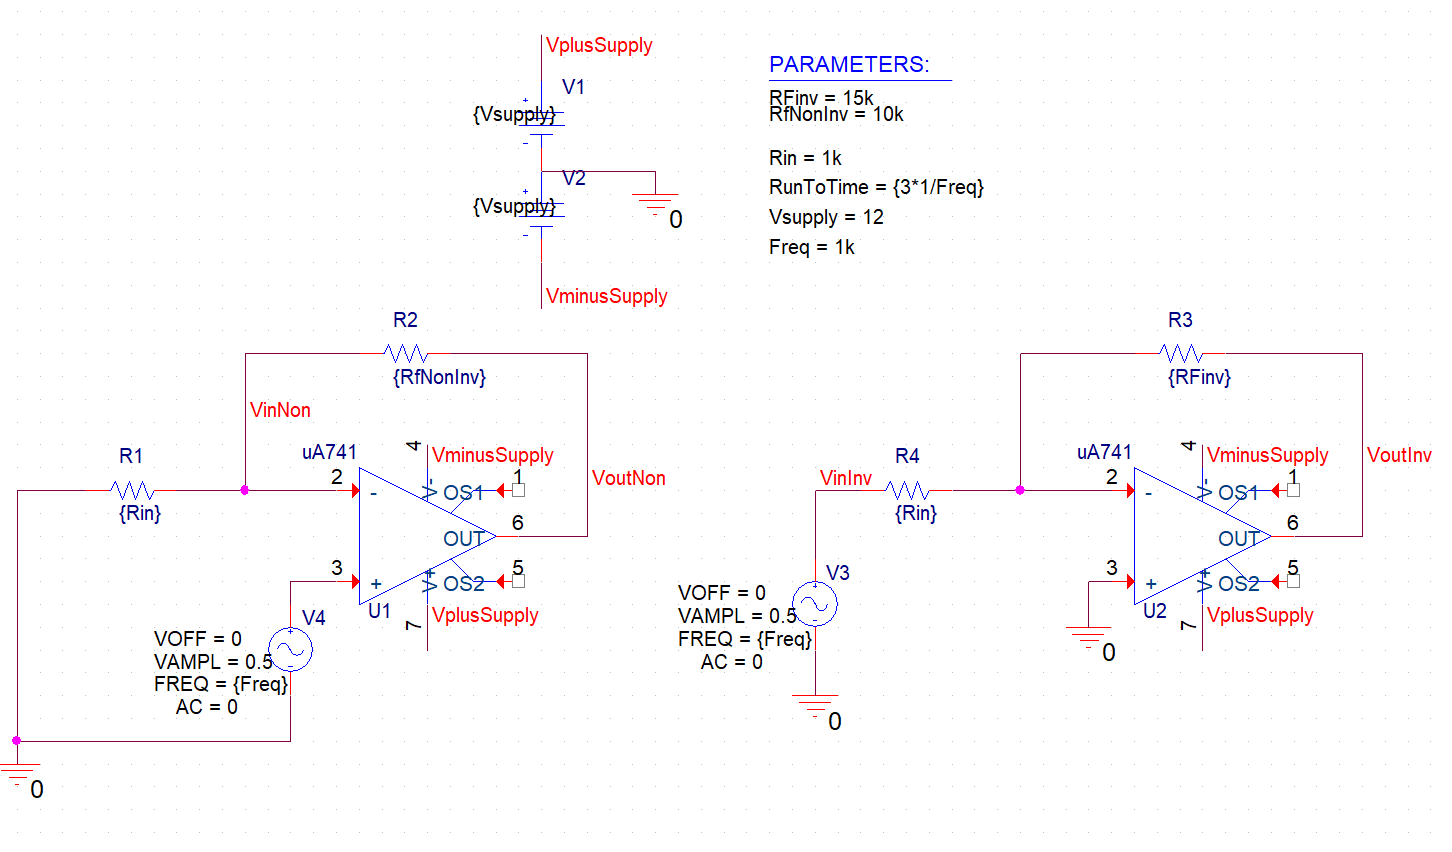
\includegraphics[width=\textwidth]{schematic}
	\caption{Schematic diagrams of the inverting (right) and non-inverting (left) OpAmps used in this report. This graphic is the PSPICE schematic capture.}
	\label{Fig:PSPICEOpAmpsGraphic}
\end{figure}

%If the data collection has deviated in any way from the rest of your section (for example you had to come back to collect more data), explain this in a second paragraph.  In particular, be sure to note if your data was acquired from a different lab than your classmates/using different equipment. 

Here two op-amps are shown. The left one is a non-inverting meaning that the gain will be a positive number. This means that the output voltage will non be a negative multiple of the input. Net-alias nodes were used to simplify the wiring of both circuits. Two $12\,\si\volt$ supplies were wired in series to then connect to the power nodes on each op-amp.

\subsection{Hand Calculations: Inverting Op-Amp}

The inverting op-amp has a desired gain of 15. The value of $V_{in}$ is an arbitrary test value that will be used to produce a ratio, this value is set $1\,\si\volt$.

\begin{align}
\label{eq:non}
V_{in} = 1\,\si\volt\\
\frac{V_{out}}{V_{in}} = -15.0\\
V_{out} = -15\,\si\volt\\
i_{in} = \frac{0\,\si\volt - V_{in}}{1\,k\si\ohm} = -1\,m\si\ampere\\
V_{out} - i_{in} \cdot R_f = 0\,\si\volt\\
-15\,\si\volt - (-1\,m\si\ampere) \cdot R_f = 0\,\si\volt\\
R_f = 15\,k\si\ohm
\end{align}

Because this op-amp is inverting, the $\frac{V_{out}}{V_{in}}$ ratio must be $-15$ as shown in Equation 1.1.2. $i_{in}$ is the current from the test source to the negative node of the op-amp. This same current will travel through the $R_f$ resistor. The desired resistance can be calculated because the required voltage drop is known. $R_f$ is determined to be $15\,k\si\ohm$.

\begin{table}[h]
	\centering
	\caption{$R_1$ and $R_f$ selection  for the Inverting Op Amp}.
	\label{Table:Lab4InvertingOpAmpSelection}
	%\begin{tabular}{llllll}
	\begin{tabular}{|c|c|c|c|}
		\hline
		$R_{in}$ (\si{\ohm})& %$I_{sc}$ (\si{\milli\ampere}) &
		$R_{f}$ (\si{\ohm}) \\
		\hline
		1k & 15k \\	 \hline 
	\end{tabular}
\end{table}
\subsection{Hand Calculations: Non-Inverting Op-Amp}

Looking at the non-inverting op-amp in Figure \ref{Fig:PSPICEOpAmpsGraphic}, the voltage on the negative terminal is equal to the one on the positive. If the input source voltage is set to the arbitrary value of $1\,\si\volt$, the $V_{in}$ node is also $1\,\si\volt$.

\begin{align}
\label{eq:non}
V_{in} = 1\,\si\volt\\
\frac{V_{out}}{V_{in}} = 11.0\\
V_{out} = 11\,\si\volt\\
i_{out} = \frac{V_{in} - 0\si\volt}{1\,k\si\ohm} = 1\,m\si\ampere\\
V_{out} - i_{out} \cdot R_f = V_{in}\\
11\,\si\volt - (1\,m\si\ampere) \cdot R_f = 1\,\si\volt\\
R_f = 10\,k\si\ohm
\end{align}

We begin with the set value $V_{in}$ being $1\,\si\volt$ and the gain of the target circuit to be $11$. To find the $R_f$ value the current through this resistor must be determined. The current $i_{out}$ defines the current from the $V_{in}$ to the ground node as depicted in Figure \ref{Fig:PSPICEOpAmpsGraphic}. The current will be the same as the current going through the $R_f$ resistor. The resistance of $R_f$ is determined to be $10\,k\si\ohm$.

\begin{table}[h]
	\centering
	\caption{$R_1$ and $R_f$ selection  for the Non-Inverting Op Amp}.
	\label{Table:Lab4NonInvertingOpAmpSelection}
	%\begin{tabular}{llllll}
	\begin{tabular}{|c|c|c|c|}
		\hline
		$R_{in}$ (\si{\ohm})& %$I_{sc}$ (\si{\milli\ampere}) &
		$R_{f}$ (\si{\ohm}) \\
		\hline
		1k & 10k \\	 \hline 
	\end{tabular}
\end{table}

\subsection{Theory: PSPICE Simulation Summary}
%Begin by providing a 1 paragraph description of the PSPICE setup. Was a DC simulation used, transient simulation, etc.?  Which \textbf{libraries} and \textbf{PSPICE elements} were used in the simulation? You can borrow from the text of your first tech memo here.  If you do so, please be sure to cite the tech memo. Note the libraries used. You can find the information when you look at the properties of each element.  There will be a reference to a ``.olb'' file.  This is the library name. 

The PSPICE simulation began with a design of the circuit. The PSPICE setup used the libraries imported from the Circuits 1 library from the lab computer. The libraries were called \textbf{analog.olb}, \textbf{opamp.olb}, \textbf{source.olb}, and \textbf{special.olb}. The components used were ``R/ANALOG'' from the \textbf{analog.olb} for the resistors, ``VDC/SOURCE'' and ``VSIN/SOURCE'' from the \textbf{source.olb} for the voltage source, ``O/CAPSYM'' and ``PARAMETER/SPECIAL'' from the \textbf{special.olb} for ground and ``ua741/OPAMP'' from \textbf{opamp.olb} for the op-amp.\\

The Vsin supply is a power source that provides a sinusoidal voltage supply. The DC offset is the phase shift of the start of the sinusoid. VAMPL is the amplitude of the sinusoid with is set to $0.5$ so that the range of the input sinusoid is $1\,\si\volt$. Finally the FREQ is the frequency with is parameterized so ease of change. The parameter RunToTime is useful to in the transient simulation to set how long the simulation should run for. In this case $\frac{3}{\{freq\}}$ will run the simulation for 3 oscillation periods.

%Include a description of the Vsin supply that was added to the circuit.  Specifically idenitify the values of the DC Offset, VAMPL, and, frequency selected.  Explain the settings used for the transient simulation.  What was the \textbf{Run to Time} value chosen to be (Note that the handout for Spring 2018 demonstrates the RunToTime parameter-how is it related to the frequency)?  Why?

\subsubsection{PSPICE Simulation: Inverting OpAmp}
%\begin{itemize}
%	\item Show the transient simulation for the inverting OpAmp 
%	\item Make sure that the input  and output waves are clearly visible.
%	\item Make the linewidth of each plot thick and clearly visible. The gain should be listed as an %extracted value per the handout's tutorial.
%	\item The figure caption should include: (i) the type of circuit (inverting opamp), (ii) the values of R1 and Rf, (iii) the peak to peak voltage of the output wave, and (iv) the resulting gain.  Please edit the figure caption below.
%	\item \textbf{A short discussion  (3 sentences) of the figure should be included, tying it back to the hand calculations. }
%\end{itemize}
\begin{figure}[h]
	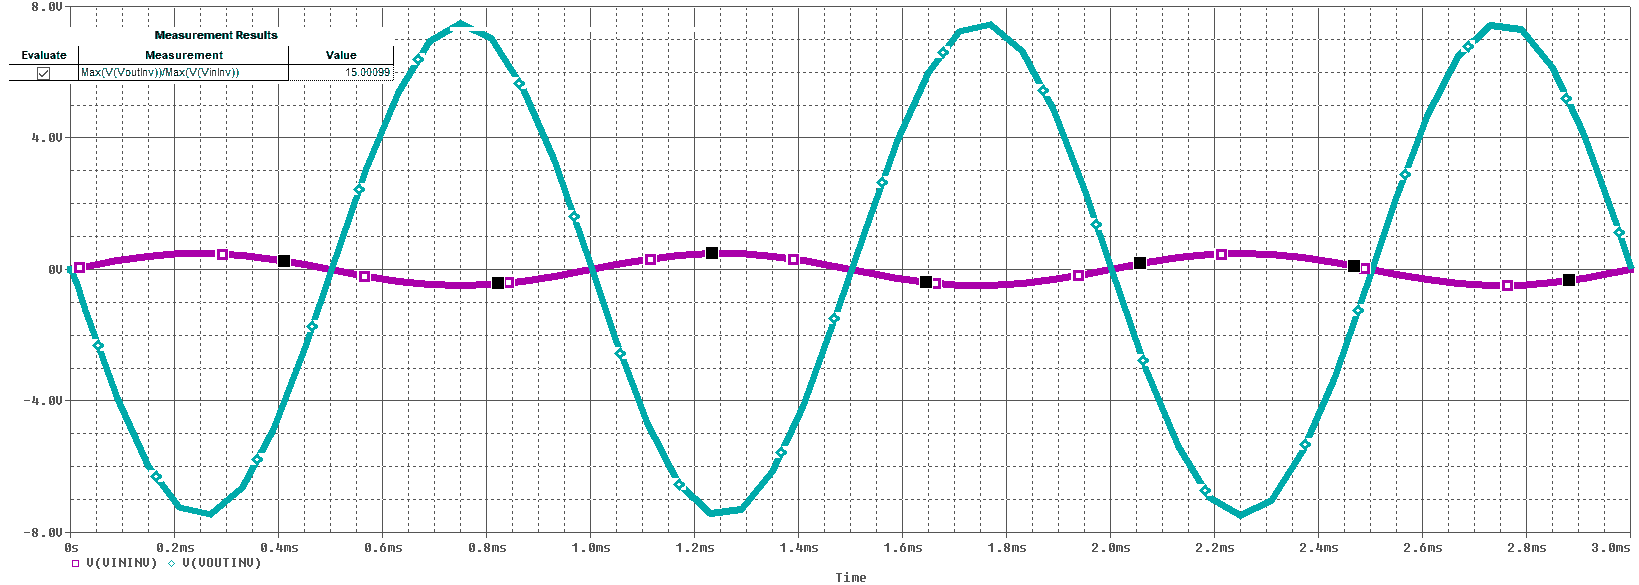
\includegraphics[width=\textwidth]{capture_inv_thick}
	\caption{Transient simulation of the inverting OpAmp.  The input wave had a peak-to-peak voltage of $1\,\si\volt$, the output wave had a peak-to-peak voltage of $15\,\si\volt$, and the gain was $15$.}
	\label{fig:capture_inv}
\end{figure}

The inverting op-amp circuit was simulated by placing a probe on the input node and the output node. This generated two sinusoids as shown in \ref{fig:capture_inv}. The gain was an measurement evaluation of the maximum peak of the output wave over the maximum on the input wave. This yieled a measured gain of just over $15$. This indicates that the calculated $RF_{inv}$ resistor was correct. The amplitude of the waves are inverted in sign which is expected from the inverting op-amp.

\pagebreak

\subsubsection{PSPICE Simulation: Non-Inverting OpAmp}
%\begin{itemize}
% 	\item Show the transient simulation for the non-inverting Op Amp 
% 	\item Make sure that the input  and output waves are clearly visible.
% 	\item Make the linewidth of each plot thick and clearly visible. The gain should be listed as an extracted value per the handout's tutorial.
% 	\item The figure caption should include: (i) the type of circuit (non-inverting opamp), (ii) the values of R1 and Rf, (iii) the peak to peak voltage of the output wave, and (iv) the resulting gain. Please edit the figure caption below.
% 	\item \textbf{A short discussion  (3 sentences) of the figure should be included, tying it back to the hand calculations. }
%\end{itemize}
\begin{figure}[h]
	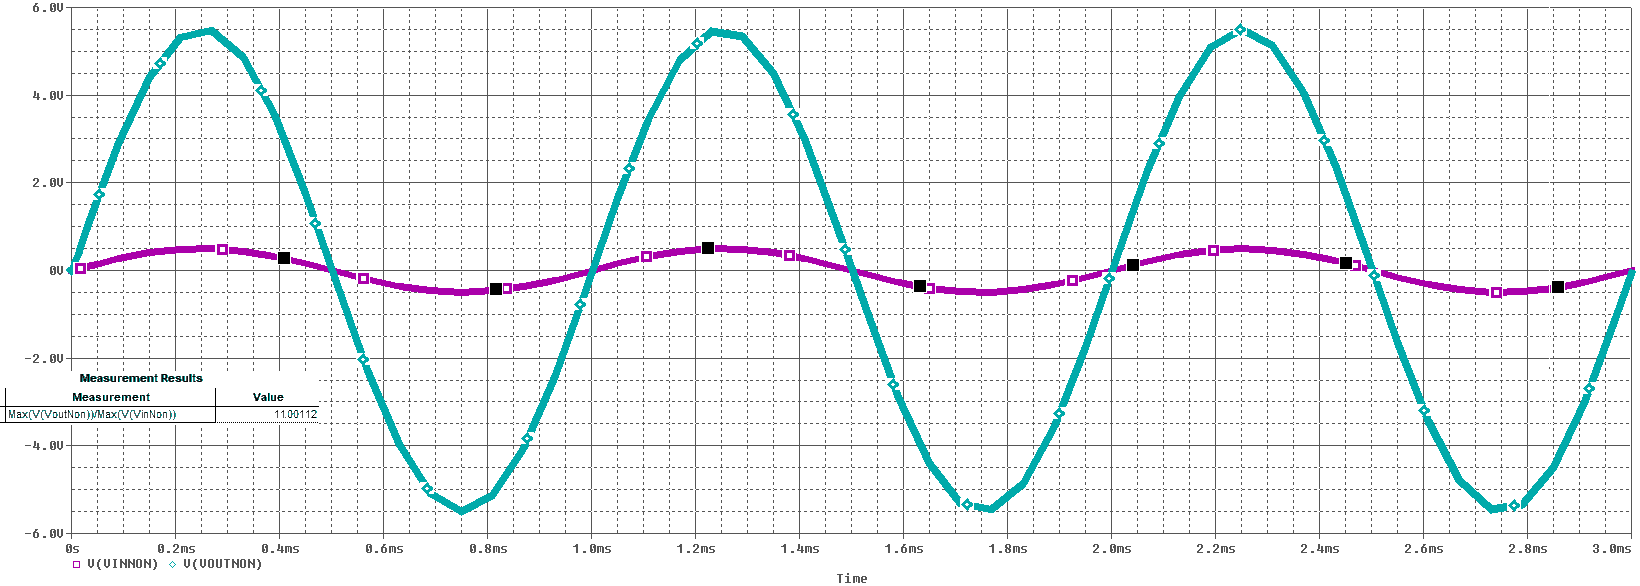
\includegraphics[width=\textwidth]{capture_non_thick}
	\caption{Transient simulation of the non-inverting OpAmp. The input wave had a peak-to-peak voltage of $1\,\si\volt$, the output wave had a peak-to-peak voltage of $11\,\si\volt$, and the gain was $11$.}
\end{figure}

The non-inverting op-amp circuit was simulated similarly to the inverting op-amp. The evaluated gain was measured to be $11$ which matches the hand calculations. The sinusoids do not have a phase shift like the inverting op-amp. The sign of the output is the same as the input as is expected in a non-inverting op-amp.

\section{Conclusion}

This laboratory experiment set up two op-amps with different gains. The PSPICE simulation showed the graph of the output and input curves generated by a sinusoidal input voltage source. The simulated circuit did not have exact gains from the calculated circuits. This is because the ideal op-amp model was used to calculate the resistor values. The slight different between the ideal and simulated op-amp accounts for this difference. In this configuration no clipping occures because the peak output voltage never reaches a value above the voltage powering the op-amp. If the output gain were to bring the output voltage above this value, the output sinusoid would reach a ceiling at this value. If the power supply voltage was adjusted to $15\,\si\volt$, the both of the op-amps would peak at $15\,\si\volt$ if the input voltage were to bring it that high.

%Provide a 1 paragraph summary of the laboratory experiment.  What were the major conclusions for each part of the experiment?  Also did the theory agree with the experiment?  The conclusion is a revised version of the abstract. Some specific verbiage from the lab documentation lists the following points:

%\begin{itemize}
%	\item Include a concise statement of conclusions commenting on differences, if any, between the ideal and simulated performance of the circuit and theory. 
%	\item  Does the data agree with the hand calculations and PSPICE simulations? Why does clipping occur (discuss)? How would the voltage resulting in onset of clipping change if the power supply was adjusted to +/- 15 volts for both configurations.
%\end{itemize}	

\section{Acknowledgments}

\begin{itemize}
	\item wikibooks.org helped with the \LaTeX\;code.
	\item tex.stackexchange.com helped with the circuit diagram in \LaTeX.
	\item Petre Tumbar and Walter Sigel were present for the prelab and experiment.
\end{itemize}

\begin{thebibliography}{9}
	\bibitem{AlexanderSadiku}
	C.K. Alexander, and M.K.O. Sadiku,
	\emph{Fundamentals of Electric Circuits, 4th Edition},
	McGraw Hill, pp. all slides, 2009.
	\bibitem{OldLab}
A. Tumbar,
	\emph{EEEE 281 Lab 3 Tech Memo},
	all pages, submitted 2, 18, 2020.
	\bibitem{RommelLab}
	S. Rommel,
	\emph{EEEE 281 Lab 4 Lecture notes},
	all slides, Spring 2015.
\end{thebibliography}

\end{document}



